\documentclass{standalone}
\usepackage{pgf}
\usepackage{amsmath}
\usepackage{tikz}
\usetikzlibrary{shapes,arrows}
\usetikzlibrary{positioning}
\begin{document}
   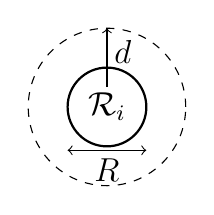
\begin{tikzpicture}[
    node distance = 0mm,
every node/.style = {inner sep=2pt}]
\coordinate  (a) at (0,0);
\coordinate  (b) at (0,1);
\coordinate (c) at (0.5,0);
 
\draw[thick] (a) circle (0.5cm);


\draw[dashed] (a) circle (1cm);
\node (a) {\large $\mathcal{R}_i$};

\draw [arrows=<->] (-0.5,-0.55) -- (+0.5,-0.55);
\node[draw=none,align=left] at (0,-0.80) {\large $R$};

\draw [->] (a) edge (b);
\node[draw=none,align=left] at (0.2,0.70) {\large $d$};
\end{tikzpicture}
\end{document}




